\chapter{Introduction}
\label{chapter-introduction}

\pagestyle{fancy}
\setcounter{page}{1}
\pagenumbering{arabic}

%Overview of petroleum engineering projects
The exploration and production of oil and gas are essential activities for fulfilling the needs of contemporary society.
%
Delivering those resources is often associated with projects of high costs and risks.
%
A standard way to mitigate those risks and maximize return on investment is to utilize reservoir models, which allows decision-makers to evaluate the economic viability of their projects and select the best strategies for their development.
%
The process of building and updating those models is broad and multidisciplinary, requiring data from different sources including seismic surveys, cores, well logs, and well tests.

%What is a well test?
A well test, according to \cite{Bourdet2002},  is a formation evaluation technique that consists of monitoring the pressure of a well in production or injection during a relatively short time compared to the life cycle of the reservoir. 
%
This analysis can provide information about the reservoir and the well during a dynamic state, as opposed to geological and geophysical sources that usually only provides data of static periods.
%
The data gathered in a well test can thus be processed with interpretation techniques, generating valuable input for reservoir models.

%Well test interpretation
The well test interpretation is an inverse problem, in which the interpreter has to create or update a model based on what the output of this model has to be.
%
In other words, the interpreter has to build a reservoir model that, under flow simulation, produces similar values of pressure than the experimental data collected from the well test.
%
This process allows to determine different proprieties in the reservoir model, such as the wellbore storage factor, skin factor, permeability and flow regime.

%What is upscaling?
When numerical models are utilized to assist well test interpretations, it is usually necessary to run simulations in models with lower resolution than the geological model available, an essential practice for optimizing the usage of computational power.
%
According to \cite{Christie1996}, geostatistical algorithms can describe petrophysical proprieties of a reservoir with such a high resolution that implies in geological models being far too detailed to be utilized as grids in reservoir simulators.
%
As a result, before running numerical simulations, it is commonly necessary to upscale the geological model into a representative model with a lower resolution.
%
This process is known as upscaling and can be visualized in Figure \ref{figure-permeability-upscaling} below.
\begin{figure}[H]
	\centering 
	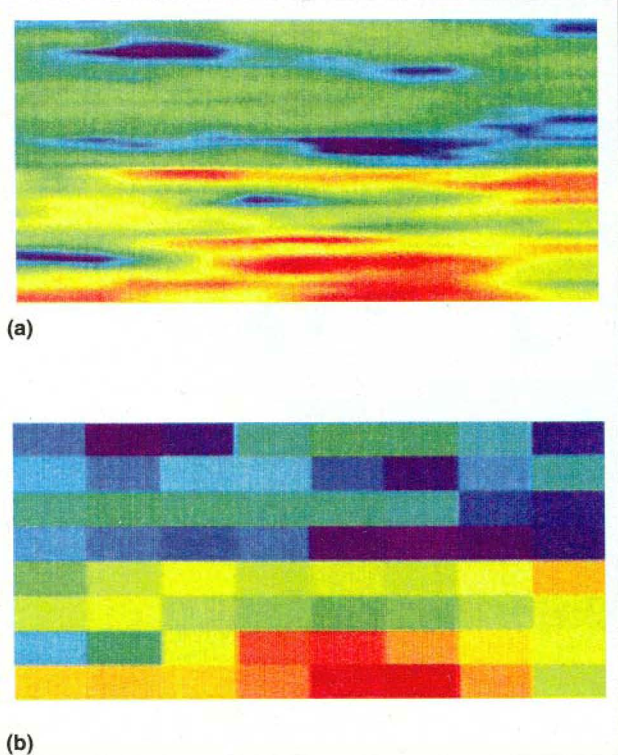
\includegraphics[width=0.5\linewidth]{Images/figure-permeability-upscaling}
	\caption{Absolute permeabilities. a) in 128x128 grid. b) in an 8x8 upscaled grid. Source: \cite{Christie1996}.}
	\label{figure-permeability-upscaling}
\end{figure}

%Why upscaling is relevant
\cite{Lie2015} states that even if one had all the computational power necessary to run simulations in high-resolution, geological models, this practice could still be ineffective for several reasons.
%
Firstly, the industry trend indicates that a surplus in computational power would enable geologists and reservoir engineers to build even larger and more complex geological models, outperforming the improvements of flow simulation capabilities.
%
Second, for many reservoir modeling workflows, it would be preferential to utilize the surplus in computational power to run more simulations in a low-resolution model, hence contemplating different development scenarios and spanning their range of plausible outputs; than performing a smaller number of simulations in a high-resolution, geological model.
%
Lastly, low-resolution models contain fewer parameters than high-resolution ones, so it is easier to calibrate them with observed data in inverse modeling workflows.

%Problems with upscaling

\section{Objectives}

This project's main objective is to analyze the effects of heterogeneity losses due to upscaling in well test simulations.
%
The idea is to build four fine-grid models and upscale those models into four coarse-grid ones.
%
Then, well test simulations will be done in each of those eight models, and the results of bottom-hole pressure, pressure drop, and Bourdet derivative will be compared and analyzed.
%
Such analysis will make possible a better understanding of the effects of upscaling in well test simulations, which could help to avoid quantitative and qualitative biases when utilizing numerical models to support well testing.

This study requires utilizing a reservoir simulator, which will be developed in this project as an intermediate objective.
%
The idea is to develop this software as an open-source tool for studies and researches in reservoir simulation.
%
It should contain the following features:

\begin{itemize}
	\item Single-phase fluid.
	\item Compressible flow.
	\item Cartesian grid.
	\item Domain comprising a vertical well.
	\item Peaceman well model.
	\item Well model supporting multiple perforated layers.
	\item Sealed reservoir as a Neumann-type boundary condition.
	\item Software developed in C language.
	\item Linearization by what \cite{Ertekin2001} describes as the simple iteration of the transmissibility terms.
	\item Sparse, unsymmetrical system of equations solved by utilizing the UMFPACK solvers, as seen in \cite{Davis1995}.
\end{itemize}
On the whole, those are the first characteristics of the reservoir simulator developed and utilized in this project, but the idea is to change or extend those features in the future for serving to other projects.
%
After developing the simulator, it will be validated by comparing its results with simulation done by industry-standard software.

Next, four fine-grid reservoir models will be created with different levels of petrophysical dispersion.
%
The first model will be homogeneous in terms of porosity and permeability.
%
From this base model, the other three models will be created with the same mean values of porosity and permeability, but with different standard deviations.
%
They will be generated by following a normal distribution for porosity and a log-normal distribution for permeability, calculated by a correlation.
%
The permeability should have vertical anisotropy, also obtained by the utilization of a correlation. 

After that, the bottom-hole pressures will be calculated by putting those eight models under flow simulation.
%
The simulation scenario will be the drawdown stage of the test of a production well.
%
The well will be initially closed, then opened with a constant flow rate until the end of the simulation.
%
Then, the pressure drop and Bourdet derivative will be calculated from the bottom-hole pressure and the elapsed time.
%
Finally, the plots of bottom-hole pressure, pressure drop, and Bourdet derivative for the eight models will be compared and analyzed.